\chapter{Background}

This chapter sets the theoretical basis for following discussion on low-rank metrics. We start with a brief mathematical introduction into distance metrics. Then we outline the characteristics of the Mahalanobis-like metric. At the end of the chapter we review some of the most prominent work in the area. The method we study, Neighbourhood Component Analysis (NCA), is presented in chapter \ref{ch:nca}.

\section{Theoretical background}
\label{sec:theoretical-background}
  A distance metric is a mapping from a pair of inputs to a scalar. Let $d(x,y)$ denote the distance function between the arguments $x$ and $y$. We say that $d$ is a metric if it satisfies the following properties for any $x,y,z$:
	\begin{itemize}
		\item Non-negativity: $d(x,y) \ge 0$.
		\item Distinguishability: $d(x,y)=0 \Leftrightarrow  x\equiv y$.
		\item Symmetry: $d(x,y)=d(y,x)$.
		\item Triangle Inequality: $d(x,y)\leq d(x,z) + d(z,y)$.
	\end{itemize}
	
	Essentially, a metric can be defined on any set of objects. The distance metric is valid as long as the above properties hold for any elements in the set. However, for the scope of our applications we limit ourselves to points in $D$ dimensional real space. The inputs will be represented by column vectors $\xB,\yB \in \mathbb{R}^D$. In this case the distance $d$ is a function from $\mathbb{R}^D\times\mathbb{R}^D$ to $\mathbb{R}$. A well known example of such a function is the Euclidean metric. This is defined by:
	\begin{align}
		 d(\mathbf{x},\mathbf{y}) = \sqrt{(\mathbf{x-y})\tr(\mathbf{x-y})}, \quad\mbox{with }\mathbf{x,y}\in \mathbb{R}^D.
	\end{align}
	
Albeit useful in many scenarios, the Euclidean metric has two properties that are problematic in machine learning applications:\footnote{\protect\url{http://matlabdatamining.blogspot.com/2006/11/mahalanobis-distance.html}}
	\begin{itemize}
		 \item{ \textbf{Sensitivity to variable scaling}. In geometrical situations, the values across all $D$ dimensions are measured in the same unit of length. In practical situations however, each dimension encodes a different feature of the data set. The Euclidean metric is sensitive to scaling and it returns different results if we change the measurement units for one of the $D$ variables. We compensate this differences by dividing the values on dimension~$i$ by the standard deviation~$s_i$ on that direction:
		  \begin{align}
		   d(\mathbf{x},\mathbf{y}) &= \sqrt{\left(\frac{x_1-y_1}{s_1}\right)^2+\cdots+\left(\frac{x_D-y_D}{s_D}\right)^2} = \notag\\
		   &= \sqrt{(\mathbf{x-y})\tr\SB^{-1}(\mathbf{x-y})}, \label{eq:new-distance}
		  \end{align}
		 where $\SB=\operatorname{diag}(s_1^2,\cdots,s_D^2)$ and $s_i = \operatorname{var}[x_i],\forall i=1,\cdots,D$.
		 }
		 \item{ \textbf{Invariance to correlated variables}. Euclidean distance treats equally the discrepancy across any of the $D$~dimensions. Often many features of a data set are redundant and, because of their number, they significantly influence the distance. Take the example of images and face recognition. The pixels from the image background are highly correlated and they reflect the same information: the colour of the background. If the two pictures of the same subject have different backgrounds, we get a high distance between the images. This effect is alleviated if we replace $\SB$ in equation \eqref{eq:new-distance} with the covariance matrix of the data:
		 \begin{align}
		 d(\mathbf{x},\mathbf{y}) = \sqrt{(\mathbf{x-y})\tr\SB^{-1}(\mathbf{x-y})},
		 \label{eq:mahalnobis-distance}
		 \end{align}
		 where $\SB = \operatorname{cov}[\mathcal{D}]$, $\mathcal{D}$ is the dataset. The metric defined in equation \ref{eq:mahalnobis-distance} is known as the Mahalanobis distance. %This is an extended version of the Euclidean metric which takes into account the correlation in the data.
		 }
	\end{itemize}
%A distance metric represents a function or a mapping from a pair of inputs to a scalar proportional to the dissimilarity of the inputs. Additionally, in order to be a proper distance, the given function ought to be non-negative, symmetric and it should respect the triangle inequality. The most common and used metric is the standard Euclidean distance. It often appears and is very useful in many geometrical situations, when distances between points need to be calculated. However, it has two major drawbacks that are problematic especially in machine learning applications. First of all, Euclidean distance is sensitive to scaling. Whilst in mathematical problems this does not constitute an issue, in real situations, we may have features that are measured in different units (e.g., seconds, kilograms, etc.) and we will obtain different distances between our data points if we change the scalings on some axis. The other problem is the fact that it does not take into consideration the correlations in the data structure. It can often happen that more attributes reflect the same information present in the data and, consequently, the distance is strongly influenced by those attributes. Take the example of face recognition: there the pixels from the image background are highly correlated and they usually reflect the same information, i.e., the colour of the background.

%The standard notation is $d(\mathbf{x},\mathbf{y})$ and it represents a function that calculates the distance between two inputs $\mathbf{x}$ and $\mathbf{y}$ (column vectors in a $D$ dimensional space $\mathbf{x},\mathbf{y}\in \mathbb{R}^D$). Essentially, the metric maps a pair from $\mathbb{R}^D\times \mathbb{R}^D$ to a real number scalar. 

%Formally, $d:\mathbb{R}^D\times \mathbb{R}^D \to \mathbb{R}$ is a metric if for any $\mathbf{x,y,z}\in \mathbb{R}^D$ the following properties hold: %\cite{Kochanski2009}
%\begin{itemize}
% \item Non-negativity: $d(\mathbf{x},\mathbf{y}) \ge 0$.
% \item Distinguishability: $d(\mathbf{x},\mathbf{y})=0 \Leftrightarrow  \mathbf{x}=\mathbf{y}$.
% \item Symmetry: $d(\mathbf{x},\mathbf{y})=d(\mathbf{y},\mathbf{x})$.
% \item Triangle Inequality: $d(\mathbf{x},\mathbf{y})\leq d(\mathbf{x},\mathbf{z}) + d(\mathbf{z},\mathbf{y})$.
%\end{itemize}

%Now we can relate the previous definition with the most common and used example: Euclidean distance. This is defined as:
%\begin{align}
% d_E(\mathbf{x},\mathbf{y}) = \sqrt{(\mathbf{x-y})^T(\mathbf{x-y})}, \mbox{ with }\mathbf{x,y}\in \mathbb{R}^D.
%\end{align}

%Unfortunately, the Euclidean distance has two major drawbacks that are problematic especially in machine learning applications\footnote{\url{http://matlabdatamining.blogspot.com/2006/11/mahalanobis-distance.html}}:
%\begin{itemize}
% \item{ \textbf{Sensitivity to variable scaling}. In geometrical situations, all variables are measured in the same units of length; for some of the real data variability is stronger on certain dimensions than on others. Naturally, we try to compensate the acute difference; so we want components with high variability to receive less weight than those with low variability. We can obtain this by simply rescaling the components with corresponding values $(s_i)_{i=\overline{1,D}}$: 
%  \begin{align}
%   d(\mathbf{x},\mathbf{y}) &= \sqrt{\left(\frac{x_1-y_1}{s_1}\right)^2+\cdots+\left(\frac{x_D-y_D}{s_D}\right)^2} = \notag\\
%   &= \sqrt{(\mathbf{x-y})^TS^{-1}(\mathbf{x-y})} \label{eq:new-distance}
%  \end{align}
% where $S^{-1}=\operatorname{diag}(s_1^2,\cdots,s_D^2)$. 
% }
% \item{ \textbf{Invariance to correlated variables}. Euclidean distance does not take into account the correlations in the data structure. For face images, for example, the pixels in the background, usually have the same colour, especially if they are close to each other; if these pixels differ strongly for other picture of the same person, we will be heavily penalized, because their number is large and the distance will be influenced by them. Therefore, we should not take into account all these variables since they reflect the same information (i.e., the color of the background). Intuitively, we want our distance metric to reflect the correlation in the data. This can be easily achieved by replacing $S$ in Equation \eqref{eq:new-distance} with the covariance matrix of the data.
% \begin{align}
% d(\mathbf{x},\mathbf{y}) = \sqrt{(\mathbf{x-y})^TS^{-1}(\mathbf{x-y})}, \mbox{ with } S = \operatorname{cov}(\mathcal{X})
% \label{eq:mahalnobis-distance}
% \end{align}
% where $\mathcal{X}$ is the dataset $\mathcal{X}=(\mathbf{x}_i)_{i=\overline{1,N}}$. 
% }

	\begin{figure}
		 \centering
			  \subfigure[Face recognition]{\label{fig:face-recog}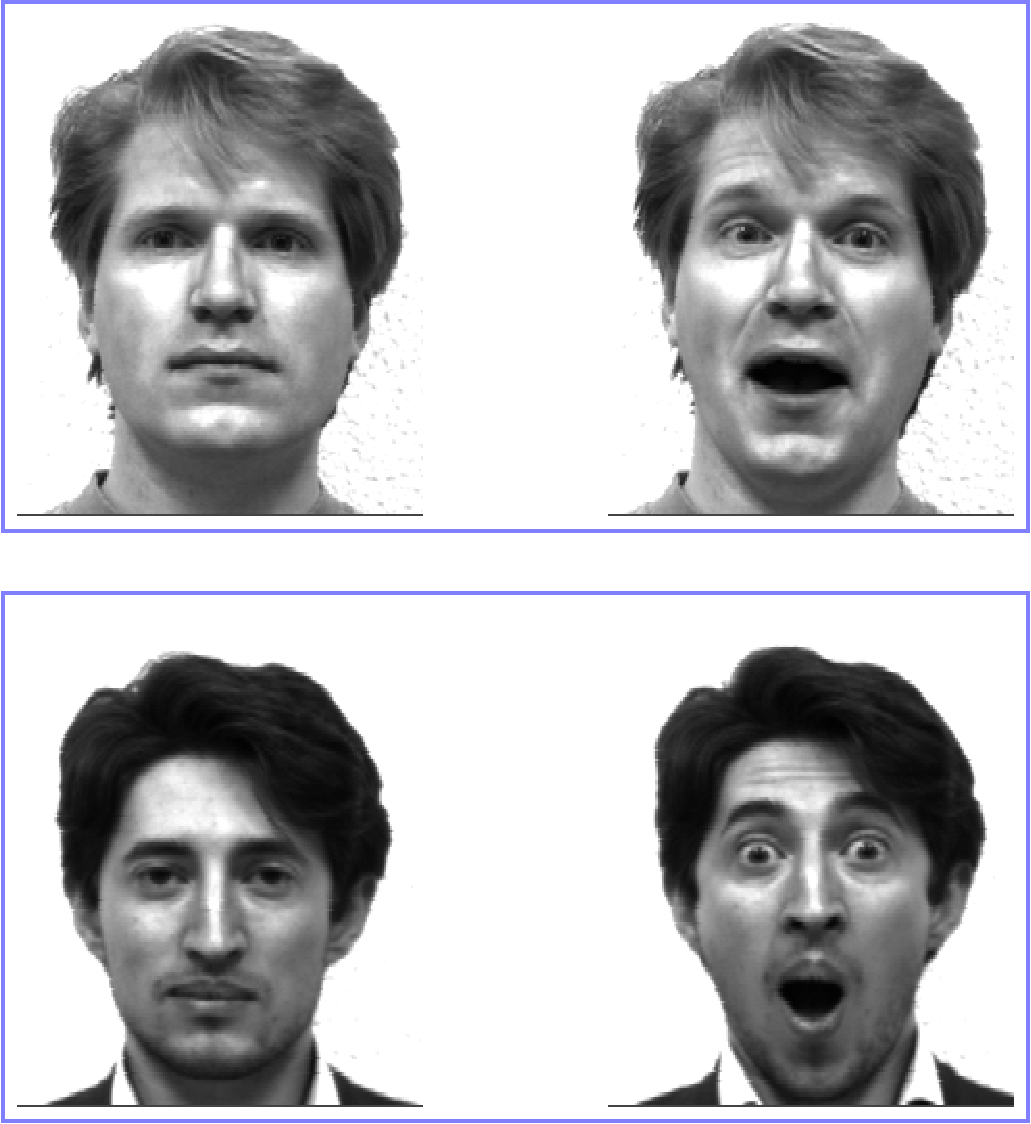
\includegraphics[width=0.48\textwidth]{images/face-recog}}
			 \subfigure[Expression recogntion]{\label{fig:expression-recog}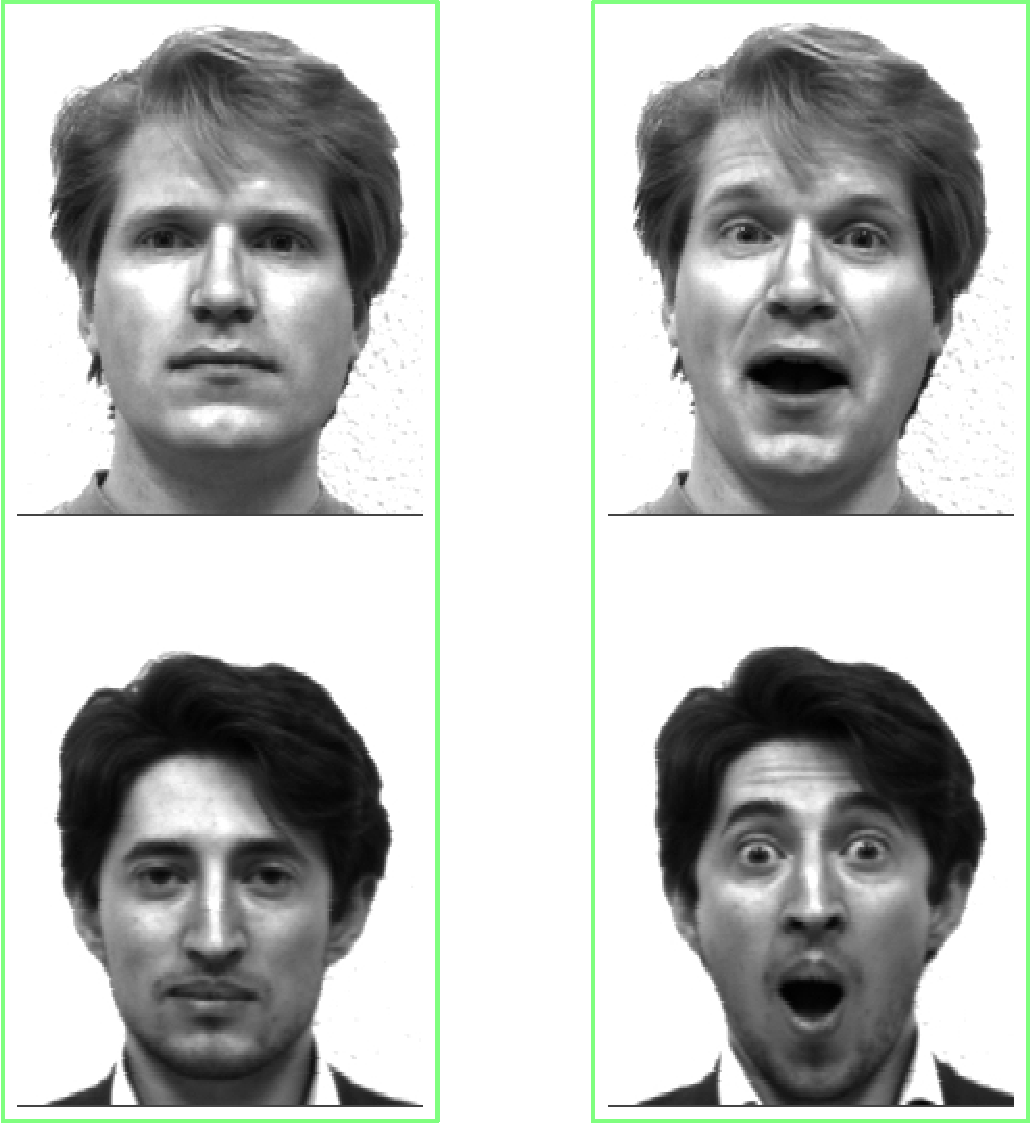
\includegraphics[width=0.48\textwidth]{images/expression-recog}}
		\caption{On a given data set we might need to perform multiple tasks; in this example: face recognition and expression recognition. Euclidean metric is not optimal since we want different pairs of equivalence for the two tasks. A good distance metric should be task dependent. These images are an extract from ORL database.}
		\label{fig:face-recog-vs-expression-recog}
	\end{figure}

The Mahalanobis metric extends the Euclidean distance by incorporating data specific information. But a good metric should be even more flexible than that. Apart for the data set, we are also given a task to perform. We want our metric to extract and discriminate only between information that is relevant to our given task. Again, in the face
recognition example we are not interested at all in
the background colour so the importance of that feature
should be down-weighted. In figure \ref{fig:face-recog-vs-expression-recog}, we illustrate that for a given data set it is not optimal to use a fixed metric.

We can further generalize the result from equation \ref{eq:mahalnobis-distance}.
Instead of setting $\SB$ as the covariance of the data, we let $\SB$ be a different matrix. The problem of determining a suitable matrix
$\SB^{-1}$ is called Mahalanobis (or quadratic) distance metric learning. We note that $\SB^{-1}$ ought to be positive semi-definite $\mathbf{x}\tr\SB^{-1}\mathbf{x} \geq 0, \forall\;\mathbf{x}$. This ensures that the norm is a real value: $d(\mathbf{x},\mathbf{0})\equiv\lVert \mathbf{x}\lVert = \sqrt{\mathbf{x}\tr\SB^{-1}\mathbf{x}}\in\mathbb{R}$.

%We need to further extend the previous result. Given a data set we usually do not care for the data set variance, but want to adapt the weights on the dimensions such that they suit our task. When we want to discriminate among face, we have some dimensions that 

%Equation \eqref{eq:mahalnobis-distance} is the standard definition of the Mahalanobis distance. Since we do not care for any variance in the data, but just for that is representative for our particular task (as discussed in Section \ref{sec:introduction}), we will consider different matrices $S$ that are suitable for the given query. Since we want our metric to discriminate among faces, we down-weight the less informative dimensions. 

There is an interesting equivalence between a Mahalanobis-like metric and a linear transformation. Using Cholesky decomposition we can write $\SB^{-1}=\AB\tr\AB$, which gives $\lVert \mathbf{x} \lVert = \sqrt{(\AB\mathbf{x})\tr(\AB\mathbf{x})}$, where $\AB$ represents a linear transformation of the data. Hence, the problem of finding a suitable distance metric $\SB$ is equivalent to the problem of finding a good linear transformation $\AB$ and then applying Euclidean distance in the projected space. We will discuss these two variants interchangeably and we will often parametrize our models in terms of $\AB$.

\section{Related methods}
\label{sec:related-methods}

The first attempts in metric learning were simple alterations of the Euclidean metric to improve $k$NN performance. For example, \citet{mitchell1997} suggests to weight each attribute of the data points such that the cross validation error is minimized. This technique is equivalent to stretching the axis of the relevant attributes and compressing the axis of the attributes that are less informative. The approach is similar to learning a diagonal metric, equation \ref{eq:new-distance}. Another method \citep{moore1994} is to eliminate the least relevant attributes: they are given a weight of zero. Albeit useful, these techniques are restrictive as the feature scaling does not reflect how the data covary.

\citet{hastie1996} proposed Discriminant Adaptive Nearest Neighbours (DANN), a method that constructs a local metric for each particular query. The metric is chosen such that it provides the best discrimination amongst classes in the neighbourhood of the query point. This increases the already costly testing time of $k$NN. However, DANN method provides a non-linear metric if we take into account all the possible resulted local linear distance metrics. Even though non-linear transformations represent a very interesting domain, we will concentrate our attention on linear metrics as they are less prone to over-fitting and easier to learn and represent.

\citet{xing2003} proposed learning a Mahalanobis-like distance metric for clustering in a semi-supervised context. There are specified pairs of similar data points and the algorithm finds the linear projection that minimizes the distance between these pairs without collapsing the whole data set to a single point. This approach is formulated as a convex optimization problem with constraints. The solution is attained using an iterative procedure, such as Newton-Raphson. This method assumes that the data set is unimodal and leverages the assumption-free $k$NN. Another drawback is the training time, because the iterative process is costly for large data sets.

Relevant Component Analysis (RCA; \citealp{bar2003, shental2002}) is another method that makes use of the labels of the classes in a semi-supervised way to provide a distance metric. More precisely, RCA uses the so-called chunklet information. A chunklet contains points from the same class, but the class label is not known; data points that belong to the same chunklet have the same label, while data points from different chunklets do not necessarily belong to different classes. The main idea behind RCA is to find a linear transformation which ``whitens'' the data with respect to the averaged within-chunklet covariance matrix \citep{weinberger2009}. Compared to the method of \citet{xing2003}, RCA has the advantage of presenting a closed form solution, but it has even stricter assumptions about the data: it considers that the data points in each class are normally distributed so they can be described using only second order statistics \citep{goldberger2004}.

Large Margin Nearest Neighbour (LMNN; \citealp{weinberger2009}) was designed especially for $k$NN classification. And it can be regarded as the support vector machine (SVM) counter part of metric learning techniques. LMNN also separates the classes by a certain margin and it inherits convexity property. Also it falls into the category of semi-definite programming. The authors also introduces various approaches to speed up the computations and to learn local metrics.

Metric learning is an ongoing research area in machine learning with an abundance of different techniques. For a good report that covers many related methods, the reader is referred to \citep{yang2006}.